%%%%%
%%
%% Sample document ``thesis.tex''
%%
%% Version: v0.2
%% Authors: Jean Martina, Rok Strnisa, Matej Urbas
%% Date: 30/07/2008
%%
%% Copyright (c) 2008-2011, Rok Strniša, Jean Martina, Matej Urbas
%% License: Simplified BSD License
%% License file: ./License
%% Original License URL: http://www.freebsd.org/copyright/freebsd-license.html
%%%%%

% Available documentclass options:
%
%   <all `report` document class options, e.g.: `a5paper`>
%   withindex   - enables the index. New index entries can be added through `\index{my entry}`
%   glossary    - enables the glossary.
%   techreport  - typesets the thesis in the technical report format.
%   firstyr     - formats the document as a first-year report.
%   times       - uses the `Times` font.
%   backrefs    - add back references in the Bibliography section
%
% For more info see `README.md`
\documentclass[withindex,glossary,firstyr,times]{cam-thesis}

% Citations using numbers
\usepackage[numbers]{natbib}
\usepackage[utf8]{inputenc} % allow utf-8 input
\usepackage[T1]{fontenc}    % use 8-bit T1 fonts
\usepackage{hyperref}       % hyperlinks
\usepackage{url}            % simple URL typesetting
\usepackage{booktabs}       % professional-quality tables
\usepackage{amsfonts}       % blackboard math symbols
\usepackage{nicefrac}       % compact symbols for 1/2, etc.
\usepackage{microtype}      % microtypography

\usepackage{algorithm}
\usepackage{algorithmic}
\usepackage{graphicx}
% \usepackage{subfigure}
\usepackage{xcolor}
\usepackage{comment}
\usepackage{caption}
\usepackage{subcaption}
\input{math_commands.tex}

%%%%%%%%%%%%%%%%%%%%%%%%%%%%%%%%%%%%%%%%%%%%%%%%%%%%%%%%%%%%%%%%%%%%%%%%%%%%%%%%
%% Thesis meta-information
%%

%% The title of the thesis:
\title{Latent-space disentanglement for \\ semantic image manipulation}

%% The full name of the author (e.g.: James Smith):
\author{Dan Andrei Iliescu}

%% College affiliation:
\college{St Edmund's College}

%% College shield [optional]:
% \collegeshield{CollegeShields/Christs}
% \collegeshield{CollegeShields/Churchill}
% \collegeshield{CollegeShields/Clare}
% \collegeshield{CollegeShields/ClareHall}
% \collegeshield{CollegeShields/CorpusChristi}
% \collegeshield{CollegeShields/Darwin}
% \collegeshield{CollegeShields/Downing}
% \collegeshield{CollegeShields/Emmanuel}
% \collegeshield{CollegeShields/Fitzwilliam}
% \collegeshield{CollegeShields/Girton}
% \collegeshield{CollegeShields/GonCaius}
% \collegeshield{CollegeShields/Homerton}
% \collegeshield{CollegeShields/HughesHall}
% \collegeshield{CollegeShields/Jesus}
% \collegeshield{CollegeShields/Kings}
% \collegeshield{CollegeShields/LucyCavendish}
% \collegeshield{CollegeShields/Magdalene}
% \collegeshield{CollegeShields/MurrayEdwards}
% \collegeshield{CollegeShields/Newnham}
% \collegeshield{CollegeShields/Pembroke}
% \collegeshield{CollegeShields/Peterhouse}
% \collegeshield{CollegeShields/Queens}
% \collegeshield{CollegeShields/Robinson}
% \collegeshield{CollegeShields/Selwyn}
% \collegeshield{CollegeShields/SidneySussex}
% \collegeshield{CollegeShields/StCatharines}
\collegeshield{CollegeShields/StEdmunds}
% \collegeshield{CollegeShields/StJohns}
% \collegeshield{CollegeShields/Trinity}
% \collegeshield{CollegeShields/TrinityHall}
% \collegeshield{CollegeShields/Wolfson}
% \collegeshield{CollegeShields/FitzwilliamRed}

%% Submission date [optional]:
% \submissiondate{November, 2042}

%% You can redefine the submission notice [optional]:
% \submissionnotice{A badass thesis submitted on time for the Degree of PhD}

%% Declaration date:
\date{My Month, My Year}

%% PDF meta-info:
\subjectline{Computer Science}
\keywords{one two three}



%%%%%%%%%%%%%%%%%%%%%%%%%%%%%%%%%%%%%%%%%%%%%%%%%%%%%%%%%%%%%%%%%%%%%%%%%%%%%%%%
%% Abstract:
%%
\abstract{%
  My abstract ...
}



%%%%%%%%%%%%%%%%%%%%%%%%%%%%%%%%%%%%%%%%%%%%%%%%%%%%%%%%%%%%%%%%%%%%%%%%%%%%%%%%
%% Acknowledgements:
%%
\acknowledgements{%
This thesis would not have been possible without the guidance, support, and encouragement of many individuals. I wish to express my sincere gratitude to all those who have helped me throughout my doctoral journey at the University of Cambridge.

First and foremost, I owe an immense debt of gratitude to Damon Wischik, my supervisor. Damon, you taught me the very essence of what it means to conduct research. Your guidance on structuring thoughts, formulating falsifiable claims, and communicating clearly – including the invaluable advice to always answer the question first – has fundamentally shaped my approach to academic work. Even fundamental skills, like how to take effective notes, were part of your mentorship. Your unwavering commitment to providing detailed feedback on countless drafts, demonstrating remarkable patience even when I repeated the same mistakes, was instrumental in my development. Thank you for offering me the opportunity to pursue this PhD under your supervision; it has been a privilege.

I am incredibly grateful to my fellow PhD students and collaborators: Aliaksei Mikhailiuk, Omer Nivron, Tudor Suciu, and Raghul Parthipan. Your camaraderie provided essential support through the inevitable confusion and challenges of doctoral research. Our deep discussions about ideas were intellectually stimulating, and the process of giving and receiving feedback was crucial for our mutual growth as researchers. Thank you for sharing the journey.

My time as an intern at Papercup Technologies was significantly enriched by my colleagues Zack Hodari, Tian Teh, and Devang Mohan, who also became valued co-authors. I thank them for their insightful feedback, for leading by example, and for their unwavering support throughout my internship. Working shoulder-to-shoulder on our paper was a rewarding collaborative experience.

I would like to extend my sincere thanks to my PhD examiners, Professor Devavrat Shah and Professor Pietro Lio. I am grateful that they agreed to take on this role and dedicate their time to evaluating my work. The viva examination itself was a stimulating experience, and I deeply appreciate their engaging discussion, valuable feedback, and insightful ideas, which have given me much to consider for future work.

On a personal note, I owe a huge debt of gratitude to my parents, Corina and Gabriel Iliescu. Your constant encouragement, especially during the final push to finish the PhD, was vital. Your genuine interest in my research meant the world to me, and knowing how happy you are that I have completed this journey brings me immense joy. Thank you for always believing in me.

Finally, and most importantly, my deepest and most heartfelt thanks go to my wife, Miruna Pislar. Miruna, your unwavering encouragement and support, particularly during the intense period of thesis writing, were my anchor. Your advice and feedback were invaluable, but even more so was your help in understanding why this endeavour was worthwhile. Thank you for giving my life colour and for being my constant source of strength and inspiration throughout this entire process.
}



%%%%%%%%%%%%%%%%%%%%%%%%%%%%%%%%%%%%%%%%%%%%%%%%%%%%%%%%%%%%%%%%%%%%%%%%%%%%%%%%
%% Glossary [optional]:
%%
\newglossaryentry{HOL}{
    name=HOL,
    description={Higher-order logic}
}



%%%%%%%%%%%%%%%%%%%%%%%%%%%%%%%%%%%%%%%%%%%%%%%%%%%%%%%%%%%%%%%%%%%%%%%%%%%%%%%%
%% Contents:
%%
\begin{document}



%%%%%%%%%%%%%%%%%%%%%%%%%%%%%%%%%%%%%%%%%%%%%%%%%%%%%%%%%%%%%%%%%%%%%%%%%%%%%%%%
%% Title page, abstract, declaration etc.:
%% -    the title page (is automatically omitted in the technical report mode).
\frontmatter{}



%%%%%%%%%%%%%%%%%%%%%%%%%%%%%%%%%%%%%%%%%%%%%%%%%%%%%%%%%%%%%%%%%%%%%%%%%%%%%%%%
%% Thesis body:
%%
\chapter{Introduction}

% \textbf{<<Some introductory sentences about image manipulation here>>}

The problem I wish to tackle in my PhD is how to learn unsupervised representations of images which naturally separate shape and appearance and segment along the lines of the image components (objects in the scene), in order to allow for easy insertion, removal and manipulation of the constituent objects while preserving the coherence and appearance of the image. Or, conversely, to allow for the modification of the appearance (lighting, texture, environment etc) without modifying the structure of the image components. By unsupervised, I mean that there should be absolutely no additional information given to the algorithm during training apart from the simple dataset of images itself.

\section{Proposed approach}

\begin{figure}
    \centering
    \captionsetup{format=hang}
    \includegraphics[width=0.8\textwidth]{figures/proposed_no.pdf}
    \caption{Outline of the proposed generative algorithm for image synthesis using disentangled Domain-Content latent representations.
    \\\\
    \textbf{Pixel-wise Domain-Content:} The algorithm involves generating each pixel of the output image $\rvx_{ij}$ as a function of the domain code $\rvm$, which represents the appearance of the image, and the corresponding content code $\rvo_{ij}$, which specifies to which object in the image the pixel belongs.}
    \label{fig:proposed}
\end{figure}

\textsl{My hypothesis is that treating pixels as individual datapoints (related to each other through spatial relationships) allows one to define an implicit grouping on the data (the images) with sufficient leverage to enable a learning algorithm to distinguish between shape and appearance in a fully unsupervised way.}

This statement spawns many implications about the characteristics of the intended algorithm, placing it at the intersection of multiple overlapping areas of research in machine learning and computational photography. The study of shape and appearance modelling in computer vision is extensive, providing both measurements of image statistics and generative models for image synthesis. These insights have been (mostly) reflected in the current deep learning literature, which is rather separated between methods for synthesizing appearance (style transfer, image-to-image translation) and methods for disentangling objects (object-centric representations), with a few works bridging the gap. On the other hand, the goal of representing and separating the two factors sits at the confluence of three highly inter-dependent (but not very communicative) major lines of research in machine learning: an information theoretic study of constraining and disentangling latent representations, the problem of aligning different streams of data in multivariate statistics, and work on cross-domain translation using high-capacity parametric functions (deep learning).

Because of the vast literature underpinning the components of this research question, and the often contradictory language for describing the same notions in different areas, I am attempting to start from first principles in a Bayesian probabilistic framing. There is a generative model with two types of latent variables, domain $\rvm$ and content $\rvo$, from which the image data $\rvx$ is generated \ref{fig:proposed}. The algorithm must learn the generative model, with an associated inference model, for a two-way mapping between the data and the latent representation. The meaning of the two latent variables is that the domain is a location invariant descriptor for the global appearance of the image, whereas the content is a location specific vector distributed marginally independently of the domain. These concepts have emerged from the work on disentangling representations of grouped observations that I have undergone in my first year. The logical progression in the development of the algorithm is the following:

\begin{enumerate}
    \item In my first year, I have developed a method for learning disentangled representations of domain and content from images grouped into packs with the same domain. I designed a generative model of the data and implemented it, following the paradigm of the Variational Autoencoder \cite{kingma2013auto, rezende2014stochastic}, as a deep neural architecture with an encoder parametrizing a variational approximation of the latent posterior. My model has the advantage over all other similar approaches of being able to contextualize input images within their pack of origin in order to estimate the joint distribution of the domain and content more precisely. This is a crucial feature for the Pixel-wise Domain-Content model, since most of the information of a pixel does not reside in its values but in its relationship with all the other pixels in the pack (in this case, the image).
    
    \item The next step is the pixel-wise Domain-Content algorithm (Figure \ref{fig:proposed} a)) which applies the Domain-Content principle on groups of pixels (the image itself). There is one domain representation for each image, and one content representation for each pixel. One could modify the appearance of the image by interpolating in the domain-space or modify the presence and nature of an object by painting with a particular value on the content map.
\end{enumerate}

Apart from qualitative judgement, the algorithms would require extensive validation with a variety of metrics, reflecting the research areas at whose intersection this project lies. The method of choice in image synthesis and manipulation is to run a user-study on the results of the proposed algorithm compared to the state-of-the-art methods for various tasks (inpainting, translation, image composition etc). There are also no-reference metrics for automatic image quality assessment. From the perspective of representation learning, one can estimate various statistics between the latent variable and the ground truth factor in the data which it is intended to represent. Additionally, the specific problem this project is tackling incorporates a range of subtasks with their own validation methods. For example, how correlated is the learned content map of an image with a ground truth segmentation map?

Chapter \ref{chapter:grouped} refers to the work done in my first year on Domain-Content disentanglement on grouped representations, reviewing the background knowledge and related work and contextualizing my method. Chapter \ref{chapter:next} discusses the challenges and validation methods associated with this project and suggests a research plan for the following two years.

\section{A note on notation}
\label{sec:notation}

The notation surrounding random variables and probability distributions is always problematic when it comes to machine learning. Different areas in the literature use completely different conventions regarding whether, for example, datapoints are random variables or samples from random variables, or whether there can be multiple families of distributions defined over the same random variables. For this report I have chosen the simplest notation that is also sufficiently clear for the topics discussed. 
\begin{enumerate}
    \item Each datapoint in a dataset is its own random variable, e.g. $\rvx_{i}$, and it may or may not be independent and identically distributed with the other datapoints.
    \item We can have multiple distribution families over the same variable, e.g. $p(\rvx_{i})$, $q(\rvx_{i})$.
    \item We write something like $\E_{q(\rvx_{i})} [p(\rvx_{i})]$ as shorthand for $\E_{a \sim q(\rvx_{i})} [p(\rvx_{i} = a)]$.
    \item When the $\rvx_i$ datapoints are identically distributed according to, for example, $p$, we refer to the common distribution as $p(\rvx)$, where $\rvx$ is the prototypical $\rvx_i$ variable.
    \item The notation $\underline{\rvx}_i$ refers to a set (or pack) of $\rvx_{ij}$ variables.
\end{enumerate}


\chapter{Modelling grouped observations}
\label{chapter:grouped}

% The problem of disentangling representations of grouped observations has been posed in various forms over the years in statistical and machine learning research. It involves two simultaneous conditions: i) that the information within the group is accumulated in the representation, ii) that

% \section{Deep latent variable models}

\section{An information-theoretic view of representation learning}

In their seminal work on representation learning, \citet{bengio2013representation} postulated that ``a good representation is one that captures the posterior distribution of the underlying explanatory factors of the observed input''. I believe this statement reflects a mainstream belief in the machine learning community that, ultimately, representations should reflect the parameters of the true data generating process. This would allow us to understand those parameters and/or to modify them for the synthesis of new data samples with predefined features. 

However, in the absence of a supervision signal from the true data generating process, any algorithm requires strong priors in order to learn a useful representation \cite{locatello2019challenging}. We implicitly suggest these priors when we formulate desirable properties of the representations. These usually involve either notions about the structure of the latent space (linearity, symmetry, orthogonality, sparsity, etc), or notions about the informational content of the representations (invariance to some factors, predictiveness of some other factors, mutual information between variables, etc). As explained in \cite{bengio2013representation}, we expect these categories of properties to be correlated with eachother and with the true data generating process itself, since we assume that the natural world has an interpretable, regular structure. This view is supported by the extensive discussion by \citet{higgins2018towards} about the symmetries of the natural world and how they should be incorporated into a good representation. A review of the common desirable properties and autoencoder-based models embodying them has been compiled by \citet{tschannen2018recent}.

One of the most discussed and intriguing desirable properties of latent representations is disentanglement. In the most general sense, this can be defined as the property that the latent representation can be split into parts such that each part corresponds to one separate generative factor. What this means in practice is the subject of this section. Disentanglement has been variously equated to marginal independence between the parts of the representation \cite{ver2014discovering, kim2018disentangling, chen2018isolating, kumar2017variational}, sparsity of the representation \cite{mathieu2019disentangling}, that the marginal distribution of the latent would match a pre-defined prior \cite{tolstikhin2017wasserstein, makhzani2015adversarial}, and how predictive each latent unit is of its assigned generative factor \cite{higgins2016beta, kim2017learning}. \citet{locatello2019challenging} have shown that none of these approaches is a general guarantee of success, since there is no such thing as a universal representation, and that the chosen priors should be specifically designed for the task in hand.

Observing this conclusion, I chose a specific interpretation of disentanglement for the domain-content problem: given a pack of datapoints from the same domain $\underline{\rvx}$ and the source datapoint $\rvx$ coming from that pack, find its domain $\rvm$ and content $\rvo$ variables, for which the mutual information between the variables and the source datapoint is maximized $\max I(\rvx ; \rvm, \rvo)$, the mutual information between the domain and the pack is maximized $\max I(\rvm ; \underline{\rvx})$ and the mutual information between the content and the pack is minimized $\min I(\rvo ; \underline{\rvx})$. This property is vague and not directly optimizable, but it serves as an intuitive goal for research. This interpretation springs from an information-theoretic view of disentanglement that relies on balancing of the amount of mutual information between the variables of the system.

\subsection{Information bottleneck}

The information-theoretic view of representation learning revolves around the principle of the information bottleneck (IB) \cite{tishby2000information}, which claims that a representation should contain the minimum amount of information sufficient to predict the target variable. More formally, if $\rvx$ is a source variable and $\rvy$ is a target variable, we want to find the intermediate representation $\rvz$ that follows the Rate-Distortion function of Shannon and Kolmogorov \cite{cover1999elements}:

\begin{align}
    R(\delta) = ~ &\underset{\rvz}{\min} ~ I(\rvx; \rvz) ~ \text{subject to} ~ H(\rvy | \rvz) \leq \delta \\
    &\text{where} ~ I(\rvx; \rvz) = \KL[p(\rvx, \rvz) || p(\rvx) p(\rvz)] ~ \text{(mutual information)} \\
    &\text{and} ~ H(\rvy | \rvz) = H(\rvy, \rvz) - H(\rvz) ~ \text{(conditional entropy)} \\
    &\text{and} ~ H(\rvy, \rvz) = - \E_{p(\rvy, \rvz)} [\log p(\rvy, \rvz)] ~ \text{(joint entropy)} \\
    &\text{and} ~ H(\rvz) = - \E_{p(\rvz)} [\log p(\rvz)] ~ \text{(entropy)}
\end{align}
This means ``find the representation which minimizes the mutual information between itself and the input (rate), whilst simultaneously keeping the conditional entropy of the target (distortion) under a specified amount $\delta$''. This specification corresponds to a compression-type situation, where we are trying to tighten the rate without surpassing a threshold level of distortion. \citet{tishby2000information} reformulate this as an unconstrained optimization problem by introducting a Lagrange multiplier $\beta$:

\begin{equation}
    \underset{z}{\min} ~ I(\rvx ; \rvz) + \beta H(\rvy | \rvz)
\end{equation}
This setting displays the general form of the rate-distortion trade-off, which one can reduce in either of its two compression-type or prediction-type dual forms. It also corresponds to the notion of a minimal sufficient statistic \cite{bahadur1954sufficiency}, but where $\rvz$ is a stochastic function of $\rvx$ rather than a set of deterministic measures of the distribution of $\rvx$. A probabilistic graphical model of this setting is depicted in Figure \ref{fig:nuisance}.

Some works \cite{tishby2015deep, shwartz2017opening, achille2018emergence} have argued that modern deep learning algorithms implicitly optimize the prediction-type dual form of the IB by performing constrained maximum likelihood estimation. \citet{achille2018emergence} in particular show how the loss of a regularized neural network forms an upper-bound to the generalization (test-time) loss of the network, by reframing it as an IB Lagrangian where $\rvx$ is the training data, $\rvy$ is the true data distribution and $\rvz$ are the weights of the network. They use the data processing inequality \cite{cover1999elements} to show that:

\begin{equation}
    \underbrace{I(\rvx; \rvz | \rvy)}_{\text{amount of overfitting}} \leq \underbrace{I(\rvx; \rvz)}_{\substack{\text{term implicitly minimized} \\ \text{when regularizing}}}
\end{equation}
This is in agreement with the decomposition principle of \citet{mathieu2019disentangling} which states that a good representation should predict the target as precisely as possible without memorizing the data (there should be some overlap between the representations of similar datapoints). It also has similar implications with the claims of \citet{bengio2013representation} and \citet{bruna2013invariant} that representations should be robust to small perturbations in the input.

Other works have sought to optimize the IB Lagrangian explicitly by learning variational approximations to the mutual information terms \cite{alemi2016deep}. \citet{burgess2018understanding} and \citet{alemi2018fixing} show how the $\beta$ term in the $\beta$-VAE \cite{higgins2016beta} has the effect of controlling the rate-distortion tradeoff in a Variational Autoencoder, subsequently proposing modifications of the loss that would reflect the IB Lagrangian more fully. Most notably, \citet{alemi2016deep} (inadvertently) prove that the mutual information between the inferred latent variable and the data is upper- and lower-bounded by the two terms of the ELBO:

\begin{equation}
    \E_{q(\rvx)} \E_{q(\rvz | \rvx)} [\log p(\rvx | \rvz)] \leq I_{q} (\rvz ; \rvx) \leq \E_{q(\rvx)} \KL [q(\rvz | \rvx) || p(\rvx)]
\end{equation}

\subsection{Invariance to confounding factors}

\begin{figure}
    \centering
    \captionsetup{format=hang}
    \includegraphics[width=\textwidth]{figures/nuisance.pdf}
    \caption{Bayesian networks comparing the latent inference models of Information Bottleneck \cite{tishby2000information, achille2018emergence} and Domain-Content (mine). \textbf{IB:} Learning a representation $\rvz$ which is maximally predictive to the target variable $\rvx$ whilst minimizing its mutual information with the source variable $\rvx$. \citet{achille2018emergence} show that this is also implies minimizing its mutual information with the nuisance variable $\rvn$. \textbf{Domain-Content:} We want the inferred domain and content variables $\rvm^q, \underline{\rvo}^q$ to be maximally informative of their data generating counterparts $\rvm, \underline{\rvo}$ and minimally informative of each other's counterpart.}
    \label{fig:nuisance}
\end{figure}

Beside sufficiency and minimality, another common desirable property for a representation is invariance to the factors which are independent of the target (nuisances, or confounders), a concept which has its origins in vision science. In his classic work on visual perception, \citet{gibson2014ecological} argued that the human brain's perception of an object is invariant to a set of common imaging variables, including illumination, rotation, occlusion and noise. The notion of invariance was subsequently formalized within the framework of group theory by \citet{dodwell1983lie}. A particular line or research \cite{sundaramoorthi2009set, anselmi2016invariance} has used this group assumption to construct classes of visual features maximally invariant to illumination and rotation transformations useful for image recognition.

However, the assumption that the nuisance features have a group structure places too heavy a constrain on the representation for the purposes of image synthesis \cite{soatto2014visual}. In our case, we are interested in sufficient invariance, namely the minimal mutual information achievable in the model $\min I(\rvz, \rvn)$, or maximal insensitivity \cite{achille2018emergence}. \citet{achille2018emergence} explore the notion of invariance within the same information-theoretic paradigm of the model in Figure \ref{fig:nuisance}. They show that there always exists a random variable $\rvn$ independent of $\rvy$, both of which together can fully explain the variation in $\rvx$:

\begin{equation}
    \forall \rvx, \rvy ~ \text{s.t.} ~ \rvy \to \rvx, ~ \exists \rvn \perp \rvy ~ \text{s.t.} ~ f(\rvy, \rvn) = \rvx, ~ \text{for some deterministic function} ~ f
\end{equation}
They also use the data processing inequality \cite{cover1999elements} to prove an intriguing and intuitive result, that invariance to nuisance variables is achieved implicitly when the representation becomes sufficient and minimal:

\begin{equation}
    \underbrace{I(\rvz; \rvn)}_{\text{invariance}} \leq \underbrace{I(\rvz; \rvx)}_{\text{minimality}} - \underbrace{I(\rvz; \rvy)}_{\text{sufficiency}}
\end{equation}
This result is especially useful for our case, where we do not have direct access to any of the nuisance variables.

Learning representations invariant to nuisances has been widely explored in the realm of fair representations \cite{zemel2013learning, hardt2016equality, louizos2016variational}, where one would like to make predictions based on data unaffected by some ``unfair'' discriminating features. \citet{louizos2016variational} propose a Variational Fair Autoencoder factorizes its latent representation into ``fair'' code and ``nuisance'' code, where the latter is provided as a supervised label. The method proceeds to train the autoencoder while minimizing a penalty term based on Maximum Mean Discrepancy \cite{gretton2007kernel} between the two codes.

The most sophisticated discussion of invariance to confounding factors comes from the study of causal inference through invariant predictions \cite{peters2016causal, arjovsky2019invariant}. Also called autonomy or stability \cite{pearl2009causality}, invariance is a hallmark in causal inference, that when all direct causes of a target variable have been accounted for, a predictor from the source variable to the target variable should behave equally well across different data views. In other words, the residual error of the prediction must be independent of environment \cite{magliacane2018domain}. Invariant Risk Minimization \cite{arjovsky2019invariant} involves attempting to find a representation of the data whose predictor is in a simultaneous local minimum across all the views of the data. In this setting, the nuisance variable is the environment itself.

\subsection{Invariance within Domain-Content}

In our case, we would like each inferred representation to be maximally predictive of their true data generating counterpart, and simultaneously invariant to the other's counterpart (Figure \ref{fig:nuisance}). However, neither the true domain nor the true content values are observed, since they only manifest through the grouping in the data. Therefore, we must use the pack and the individual datapoints differentially in order to estimate mutual information relationships between the variables. For example, in order to minimize the mutual information between the inferred pack of content variables $\underline{\rvo}^{q}$ and the data generating domain variable $\rvm$, we can reduce its upper-bound using the data processing inequality \cite{cover1999elements}:

\begin{equation}
    \underbrace{I(\underline{\rvo}^q; \rvm)}_{\substack{\text{inferred content pack} \\ \text{vs true domain}}} \leq \underbrace{I(\underline{\rvo}^q; \underline{\rvx})}_{\substack{\text{inferred content pack} \\ \text{vs pack}}} = \sum_{k=1}^K \underbrace{I(\rvo^q_k; \underline{\rvx})}_{\substack{\text{individual inferred} \\ \text{content vs pack}}}
    \label{eq:content_bottle}
\end{equation}
The question remains, however, how to estimate the mutual information empirically in order to optimize this.

\subsection{Estimating mutual information}

Various methods have been proposed to estimate the mutual information between empirical samples. The most widespread classical methods assign datapoints to discrete bins on the support manifold and estimate the probability distributions numerically. Much research has gone into refining the estimations of these methods by creating adaptive bin sizes \cite{fraser1986independent} or correcting via asymptotic series the estimation's susceptibility to noise \cite{grassberger1988finite}.

One modern approach is to use K-nearest neighbours to derive an estimate \cite{kraskov2004estimating}. They use the k-th nearest datapoint in order to define a local neighbourhood, and then compute their estimate based on the total number of datapoints within the neighbourhood on each of the dimension independently. This algorithm is very attractive due to its simple, non-parametric nature, and is also shown to a correct estimation for a variety of distributions.

Variational approaches \citet{houthooft2016vime, alemi2016deep} are applicable when one of the conditional distributions between the two variables can be explicitly evaluated. The method involves applying the chain rule on the joint probability, simplifying the resulting marginal, and then replacing the other marginal with a variational prior:

\begin{equation}
    I(\rvx; \rvy) = \E_{p(\rvy)} \KL[\underbrace{p(\rvx | \rvy)}_{\text{can be evaluated}} || p(\rvx)] \leq \E_{p(\rvy)} \KL[p(\rvx | \rvy) || \underbrace{r(\rvx)}_{\text{variational prior}}]
\end{equation}

The mutual information can also be approximated through deep learning. \citet{sugiyama2012density, mescheder2017adversarial} have shown how the ratio of densities can be estimated neurally using a discriminator \cite{goodfellow2014generative}. \citet{nowozin2016f} used this method to estimate the f-divergence between empirical distribution, of which one example is the dual form of the KL-divergence \cite{nguyen2010estimating}. The Donsker-Varadhan lower bound to the KL-divergence \cite{donsker1983asymptotic} holds for any family $\mathcal{F}$ that satisfies the integrability conditions. When $\mathcal{F}$ is the set of all functions with finite outputs, then the bound is tight.

\begin{equation}
    \KL [p(\rvx) || q(\rvx)] \geq \underset{f \in \mathcal{F}, ~ f: \Omega \to \R}{\sup} \E_{p(\rvx)} [f(\rvx)] - \log \E_{q(\rvx)} \left[ e^{f(\rvx)} \right]
\end{equation}
We can estimate the lower bound of the mutual information neurally \cite{belghazi2018mutual} by implementing $f$ as a trainable discriminator.

\begin{equation}
    I(\rvx, \rvy) \geq \underset{f \in \mathcal{F}}{\max} ~ \E_{p(\rvx, \rvy)} [f(\rvx, \rvy)] - \log \E_{p(\rvx)p(\rvy)} \left[ e^{f(\rvx, \rvy)} \right]
\end{equation}
Deep InfoMax \cite{hjelm2018learning} uses this estimate as a regularization term to encourage more robust representations in autoencoders with greater discriminative power. \citet{kim2018disentangling} have also adapted this method in order to estimate the total correlation \cite{watanabe1960information} among the units of a VAE's latent representation, which is the natural extension of the mutual information to multiple variables.

\section{Shared and private variation}

\begin{figure}
    \centering
    \captionsetup{format=hang}
    \includegraphics[width=\textwidth]{figures/bayes_shared_private.pdf}
    \caption{Bayesian networks contrasting generative models based on shared-private variation against the domain-content generative model. The graphical models are modified for the purpose of comparison. One significant departure from the way CCA-based models are usually represented is that, following the notation conventions [\ref{sec:notation}], there is a separate shared latent variable $\rvz_{ik}$ for every datapoint in every view. Even though is customary to show the shared variable as being common across views, in practice, every datapoint corresponds to a different value for this variable. The depiction presented here clearly shows the inherent ambiguity of the distinction between the shared and private variables, whose separation can be made only on the basis of their priors (as opposed to the domain-content model, whose separation is structural). \\\\ \textbf{a) Bayesian CCA} \cite{klami2013bayesian} separates between the shared $\rvz_{ik}$ and private $\rvz^(i)_{ik}$ representations using the constraint of its linear mapping mechanism and the latents' view-specific and view-independent priors (here the priors also encapsulate the dimensionality of the representation). \textbf{b) MRD} \cite{damianou2016multi} adapts the shared $\rvz_{ik}$ to a shared+private $\rvz^{(i)_{ik}}$ representation using a learned view-specific weighting of the latent dimensions. The role of the weights $\omega^(i)$ is similar to the role of the domain variable. \textbf{c) Domain-Content} provides structural separation between the domain $\rvm_i$ (which summarizes the view) and content $\rvo_{ik}$ (which models the intra-view variation).}
    \label{fig:bayes_shared_private}
\end{figure}

One of the first algorithms used to represent multi-view data in a shared latent space is Canonical Correlation Analysis (CCA) \cite{hotelling1992relations, hardoon2004canonical}. Its goal is to extract linear projections of the data views in a common space where they are maximally correlated. Conceptually, the method extends principal component analysis (PCA) to a multi-view setting by selecting $K$ jointly-orthogonal 1-dimensional linear transformations of the data that maximise the correlation across data views. The resulting representation is not intended to be a causal explanation, but a distillation of the features with the strongest co-occurrence.

Some works have sought a generative interpretation of CCA that can answer questions about the latent posterior density and the data likelihood and enable sampling from the data marginal. Following the paradigm of the probabilistic framing of PCA \cite{tipping1999probabilistic}, \citet{bach2005probabilistic} have shown how the CCA solution can be interpreted as the maximum likelihood parameters of a generative model consisting of two observed variables $\rvx^{(1)}, \rvx^{(2)}$ (the views of the data) sampled from normal densities whose means are affine transformations of the value of a latent variable $\rvz$ (the representation), distributed according to an isotropic normal with a diagonal matrix. Instead of extending CCA to accommodate a more sophisticated criterion for aligning the two views, this work clarifies the generative model for which CCA does already produce a latent representation which explains the data.

\subsection{Bayesian CCA}

However, because of its single latent representation, any uncorrelated variance between the two views is treated as residual noise produced by the covariance matrices of the generative posteriors $p(\rvx^{(i)} | \rvz)$. Consequently, \citet{klami2013bayesian} propose an expanded generative model to explain the data variance more precisely, by unifying CCA with inter-battery factor analysis \cite{tucker1958inter, browne1979maximum}, a method for extracting separate shared and private representations from multi-view data. The new Bayesian CCA model has both a shared latent variable $\rvz$ and a private latent variable for each view $\rvz^{(i)}$. The generative posterior of a view now takes the form of a normal whose mean is a linear combination of its two latent variables $\rmA^{(i)} \rvz + \rmB^{(i)} \rvz^{(i)}$. The authors design an ingenious Bayesian inference technique for the parameters, which involves reframing both views as a single random variable $\rvx$ and then performing Bayesian factor analysis \cite{ghahramani2000variational} with a strong sparsity prior on the linear transformation producing the mean of the generative posterior. 

Bayesian CCA identifies two crucial issues involved in learning disentangled representations of grouped data: 
\begin{enumerate}
    \item Without the presence of a latent variable with the capacity to encode private variance, the shared representation will (wrongly) seek to explain it in cases where the shared correlations are of a smaller scale.
    \item Such a disentangled model is fundamentally unidentifiable (as it is equivalent to inferring a joint representation from the marginals) so a strong prior is needed in order to learn a useful representation.
\end{enumerate}
It addresses these issues by providing a separate variable $\rvz^{(i)}$ for each view and by using the linearity of the model and the sparsity of the prior to encourage convergence towards an appropriate representation.

Bayesian CCA is appropriate, however, only when we assume that covariance is equivalent to dependence (and variance to information content). In the study of a high-dimensional, highly non-linear and sparse data such as images, covariance and orthogonality are poor predictors of information, which is ultimately the quantity in which we are interested.

\subsection{Manifold relevance determination} 

\citet{damianou2016multi} have augmented the representation power of Bayesian CCA to accommodate arbitrarily complex mappings between the latent variables and the data. This allows the criterion for alignment to move completely past co-occurence onto representations which simultaneously maximize the marginal likelihood of the data views. The method uses a Gaussian Process latent variable model (GP-LVM) \cite{lawrence2004gaussian}, the unsupervised equivalent of a Gaussian Process regression where the source variables are unobserved and treated as low-dimensional latent variables to be trained alongside the GP parameters through maximum likelihood estimation (or maximum a posteriori estimation if we wish to impose some prior structure on the latents). The authors build upon the factorized latent structure of the ``shared'' GP-LVM of \citet{ek2008gp} and propose a model with a single shared latent representation whose dimensions are weighted selectively by each data view depending on their relevance for that particular view, thus achieving a ``private interpretation'' of the shared representation. They call this mechanism manifold relevance determination (MRD).

I have only recently come across this approach but find it very compelling. The fully Bayesian, non-parametric nature of GP-LVMs allows one to reason very clearly about the priors used for selecting an alignment, which is essential in settings where the solution space is so vast, as is the case of image synthesis. \citet{shon2006learning} have used such a shared GP-LVM model to achieve good results on the task of supervised image-to-image translation by imposing a common latent representation on pairs of images depicting different objects from the same viewpoint. It would be interesting to explore if MRD could be used to learn unsupervised I2I translation using appropriate priors (thus retrieve a joint distribution having access only to marginals). MRD is also interesting from the perspective of causal invariance \cite{peters2016causal, arjovsky2019invariant}, since there is a common latent representation whose features each view is allowed to weight differently. Perhaps features that are weighted similarly across views have learned to represent causal generative factors?

\subsection{Shared-private variation vs Domain-Content}
Representations disentangling shared and private variation have also been used successfully for image-to-image translation in the context of deep learning by \citet{gonzalez2018image}. They use a clever arrangement of reconstruction losses training view-specific encoders and decoders in order to encourage the separation of latent representations into view-exclusive and view-agnostic representations.

It is worth noting at this point that, although similar in their relationship, the notions of shared and private variation do not correspond exactly to the notions of content and domain. Content can be construed as a shared representation across views, where we would expect each view to have a similar distribution of values. We would also interpret two observations having the same content/shared representation value as being ``translations'' of each other.

However, the domain variable is a much more well-defined notion than the private representation: all members of a view have, by definition, the same domain value. Indeed, the domain can be seen as a special case of a private representation where the domain value can be said to encode a recipe for transforming the shared representation into a shared-private representation. This is virtually identical to the role of the view-specific weighting in MRD \cite{damianou2016multi}. A comparison of generative models involving these notions is presented in Figure \ref{fig:bayes_shared_private}.

\section{Unsupervised image-to-image translation}

An extensive and influential line of research with significant overlap with the domain-content problem is the task of image-to-image translation: transforming an image from a source domain to correspond to the features of a target domain. This topic has its conceptual roots in the study of unsupervised domain adaptation, or finding common representations of data between multiple domains with the same label space. The seminal work of \citet{ben2010theory} has computed an upper-bound to the classification error on the target domain of a classifier $q(\rvy | \rvx)$ trained on the source domain. I have reformulated their result probabilistically as:

\begin{alignat}{2}
    &\underbrace{\epsilon_t(q)}_{\text{target error}} \leq ~ &&\underbrace{\epsilon_s(q)}_{\text{source error}} + \E_{p_s(\rvx)} \int \underbrace{|p_s(\rvy | \rvx) - p_t(\rvy | \rvx)|}_{\substack{\text{divergence between} \\ \text{the optimal predictors}}} ~ \log q(\rvy | \rvx) d\rvy + H_{p_s} (\rvy | \rvx) \notag\\ & &&+ \int \underbrace{|p_s(\rvx) - p_t(\rvx)|}_{\substack{\text{divergence between} \\ \text{the data marginals}}} ~ \underbrace{\KL[p_t(\rvy | \rvx) || q(\rvy | \rvx)]}_{\text{target error}} d\rvx - H_{p_t} (\rvy | \rvx) \\
    &\text{where} ~ \epsilon_s(q) = && E_{p_s(\rvx)} \KL [p_s(\rvy | \rvx) || q(\rvy | \rvx)] ~ \text{(source error)}
\end{alignat}
The expression suggests that the effect of the explicit target error term on the right-hand side (which is unknown) can be undone by minimizing the pointwise absolute difference between the source and target data marginals. This gave \citet{ben2010theory} the idea to map the two domains to a common representation space (that we call $\rvz$) where the data marginals of the two domains match. Notice the similarity between this and CCA.

Various methods have been subsequently proposed in order to learn such a common representation. Domain Adversarial Networks \cite{ganin2015unsupervised, ganin2016domain} have become the mainstream method for learning domain-invariant representations in the image translation literature. The method is conceptually elegant: train a discriminator \cite{goodfellow2014generative} whose task is to classify the domain origin of a representation, and train the representation network to fool the discriminator. \citet{sohn2018unsupervised} propose a slightly more sophisticated method, whereby they learn a mapping between the representations of the two domains such that, if two datapoints belong to the same class in the source domain, than their translations will be clustered together in the target domain. They introduce a novel verification loss, instantiated by a classifier taking two latent vectors as input and trying to predict whether they should belong to the same class. This method is perfectly suited for domains with different label spaces, as it preserves the private variation of each domain whilst providing a mapping which extracts the shared variation. 

Indeed, the methods described above rely on the assumption that the shared features between the two domains are represented with equivalent frequency. If, for example, a feature is more common in one domain than in the other, it will be incorrectly assigned under the rubric of private variation (this is a problem in common with most of the methods discussed). Domain adaptation using causal inference \cite{magliacane2018domain} seeks to solve this problem by relying on invariant prediction performance instead of distribution matching in order to select features for the shared representation.

As mentioned before, the problem of learning an unsupervised shared representation is equivalent to the problem of retrieving a joint distribution from its marginals: it is unidentifiable in the absence of priors and preferences. Theoretical works on unpaired translation specifically applied to images using neural networks \cite{galanti2018role, galanti2018generalization} have concluded that the deep hierarchical structure of a neural network offers a very strong prior over the space of possible translations, enabling heuristic tricks to perform very well in practice.

And, truly, there are many heuristic tricks. One of the most popular losses to be used in image-to-image translation is the cycle-consistency loss \cite{zhu2017unpaired}. It consists of translating an image to the desired domain, translating it back, and then measuring the reconstruction loss. It encourages some consistency in the translation and is used widely in the literature \cite{liu2017unsupervised, royer2020xgan, lee2018diverse}. Most models are based on the conditional GAN paradigm \cite{mirza2014conditional}, whereby the GAN generator is conditioned on the input image when producing its translation. Other heuristics include using an adversarial loss to that the translation output belongs to the target domain \cite{taigman2016unsupervised, liu2017unsupervised, huang2018multimodal, choi2018stargan, royer2020xgan}, a reconstruction loss between the source image's latent and the target image's latent \cite{taigman2016unsupervised, royer2020xgan, liu2019few}, a noise injection to enable diverse outputs \cite{huang2018multimodal, lee2018diverse}, and even a loss for preserving relative distances between the images in the source domain and their translations \cite{benaim2018one}. All state-of-the-art image translation algorithms use residual connections in a U-Net structure \cite{ronneberger2015u} in order to separate hierarchical image features and achieve high-fidelity reconstructions.

\subsection{Disentangling style and content}

The most interesting such heuristic for our purposes, and the one most related to the structure of images, is the separation of so-called style features from content features. The seminal style-transfer model \cite{gatys2015neural, gatys2016image} was instrumental in demonstrating the power of deep learning by transplanting the low-level texture statistics of one image onto the high-level structure of another. Style-transfer optimizes the image directly by passing it through a very deep object recognition network and matching the feature statistics to those of the style image.

The separation of style and content has its origins in a vast research area around factor analysis of image. The classical work on Eigenfaces \cite{sirovich1987low} is one of the first to extract the essential components of a face and recombine them to generate new faces. They use principal components analysis on a dataset of faces to extract orthogonal eigenvectors which can be linearly combined to reconstruct, reasonably faithfully, every face in the dataset. \citet{tenenbaum2000separating} extend the single factor model to a two factor bilinear model which consists of a matrix of learned basis faces multiplied left and right with the two factor vectors to yield the output image. They achieve impressive results at separating pose and appearance in the factors, and then recombining them to generate novel images. The generalization to multiple factors, TensorFaces \cite{vasilescu2002multilinear}, achieves a detailed disentanglement of images into an arbitrary number of factor vectors using multilinear models and tensor products.

The early deep learning translation methods introduced in the previous section \cite{taigman2016unsupervised, zhu2017unpaired, liu2017unsupervised} achieve excellent separation of style and content by virtue of their deep hierarchical structure, particularly suited for separating image components \cite{ulyanov2018deep}. However, methods that exploit this structure explicitly for even greater translation precision have been developed. Adaptive Instance Normalization (AdaIN) \cite{huang2017arbitrary} is a technique of manipulating the stylistic features of a generated image directly by changing the mean and variance of the activations in some generator network layers to some inputed values. \citet{karras2019style} has shown how, by using such transformations, one can generate high-quality natural images with controllable features at every level in the generation.

The separation of style-content features that AdaIN encourages has enabled the emergence of few-shot unsupervised translation algorithms \cite{wang2019few, liu2019few}. These methods can receive packs of images from unseen styles at test-time and translate images into the novel style. They rely on translation heuristics and can produce convincing, high-resolution natural images.

\section{Domain-Content: Contextualizing observations for disentanglement}

\begin{figure}
    \centering
    \captionsetup{format=hang}
    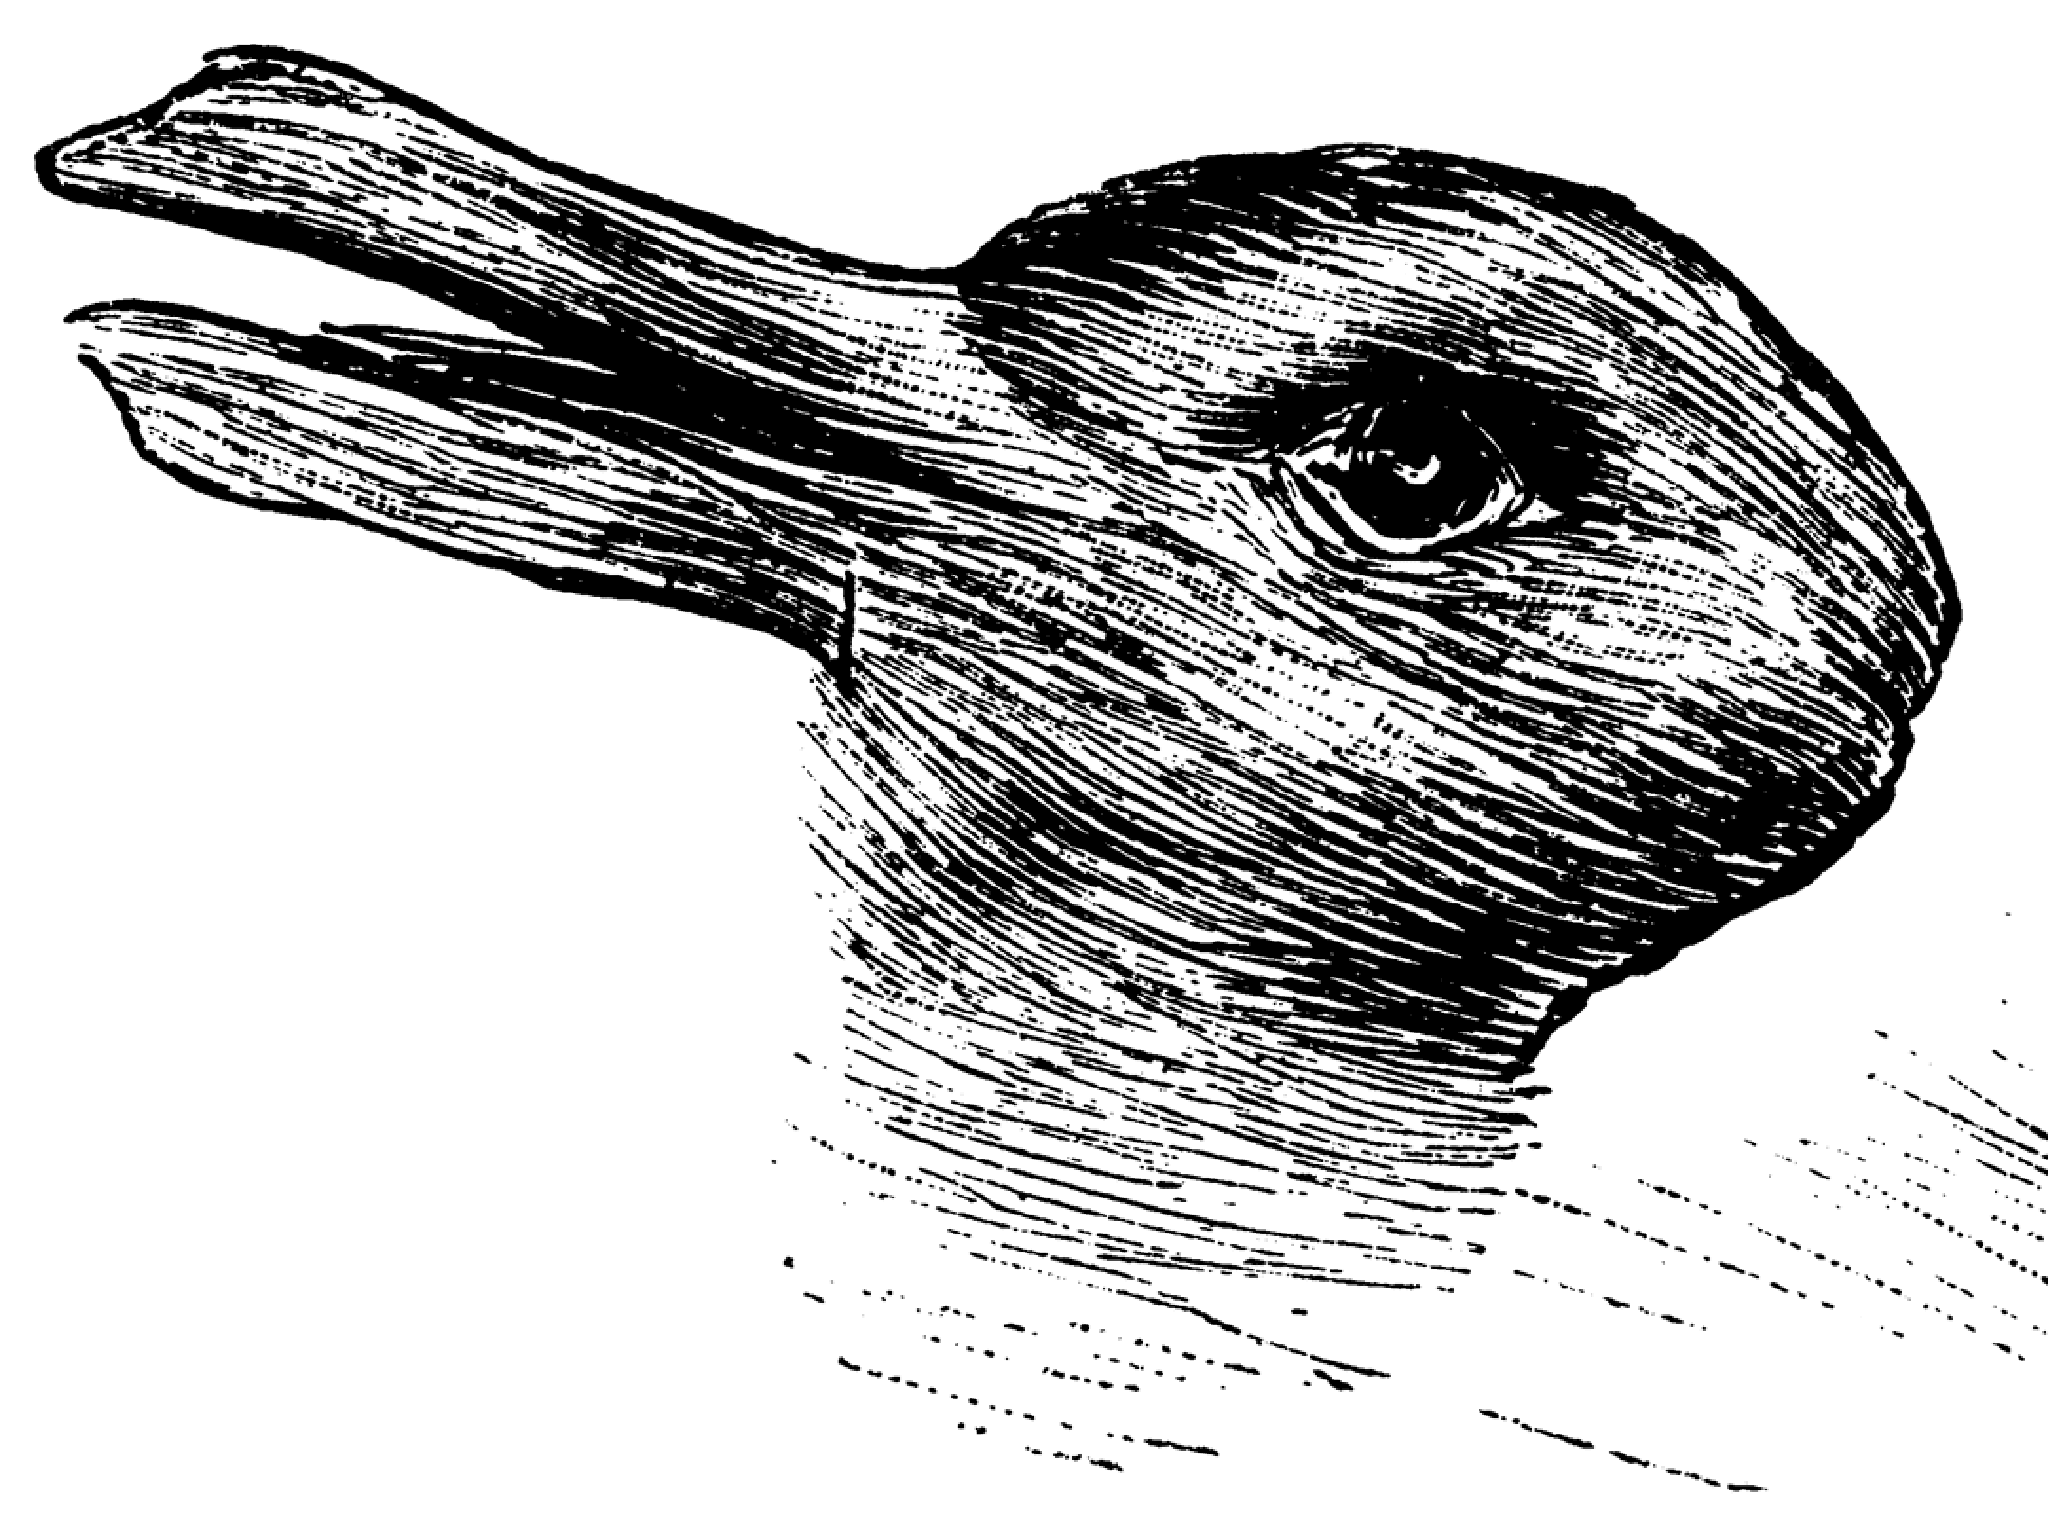
\includegraphics[width=0.5\textwidth]{figures/duck-rabbit.png}
    \caption{The famous ambiguity illusion. The pose of the animal is ambiguous in the absence of an assumed species. Changing the inferred species from ``duck'' to ``rabbit'' fundamentally changes the inferred pose. This is an (contrived) example of how the inferred content variable of an input should also be conditioned on the inferred domain variable.}
    \label{fig:duck}
\end{figure}

\begin{figure}
    \centering
    \captionsetup{format=hang}
    \includegraphics[width=\textwidth]{figures/bayes_net_new.pdf}
    \caption{Bayesian networks comparing the Domain-Content model with competing group-based disentanglement methods in the literature \cite{bouchacourt2017multi, esser2019unsupervised}. Our model is the only one whose individual-level latent inference posterior (the content) is conditioned on the group-level latent variable (the domain). This allows our latent posterior to model the joint distribution between the two latent variables conditioned on the input, and thus obtain more precise estimates. We call this ``contextualizing'' the input in its domain of origin.
    }
    \label{fig:bayes_context}
\end{figure}

\begin{figure}
    \centering
    \captionsetup{format=hang}
    \includegraphics[width=\textwidth]{figures/mo_inference.pdf}
    \caption{Impact of the domain contextualization of $\rvx' = [-1, 2]$ on the precision of the latent inference. The bottom plot depicts samples in data-space, the top plots show the encoding of $\rvx'$ into the two latent-spaces using contextualized and un-contextualized methods. The blue dots depict latent inference samples of the un-contextualized state-of-the-art model of \citet{esser2019unsupervised}. The red and orange dots depict samples from our model with $\rvx$ contextualized within two different domains. The red and orange clusters in the data plot are the two domains used for contextualizing $\rvx'$ in our method, with their respective colours. Our model's capacity for contextualization clearly increases its representation precision, especially in content-space. \\\\ \textbf{The data generation process:} The data variable $\rvx$ is a 2-d vector produced by $[\rvx_1, \rvx_2] := [\rvo_1, \rvo_2] * [\rvv, \rvv] + [\rvu, 0] + \epsilon$. $\rvo_1, \rvo_2$ are the content features (called ``$\rvx_1, \rvx_2$ displacement''), and are sampled independently from $\mathcal{N}(0, 1)$. $\rvu, \rvv$ are the domain features (called ``mean'' and ``variance'') which are sampled uniformly according to $\mathcal{U}(-3, 3), \mathcal{U}(0, 2)$ respectively. $\epislon$ is noise sampled from $\mathcal{N}(0, 0.1)$ The inherent ambiguity of this dataset (a point could have come from multiple domains) illustrates the need for contextualization.
    }
    \label{fig:mo_inference}
\end{figure}

All the methods presented so far have one crucial limitation: the content representation of each input is computed independently of its domain of origin. In the general image-to-image translation setting, the impact of this limitation is subtle as there is, usually, little overlap between domains. For example, if the task requires the model to map between faces of cats and faces of dogs, ambiguous images that could be interpreted as either cats and dogs are generally rare. Moreover, if the content in this case comprises the pose of the face, then it will almost never be the case that, if the image is interpreted as a cat, the cat would be facing to the right side of the image, if the image is interpreted as a dog, the dog would be facing to the left side of the image (though there exist some famous exceptions Figure \ref{fig:duck}).

However, when pixels become the datapoints instead of images, the datapoint itself communicates almost nothing about its content in the absence of global information about the pack. The information stored in a pixel (3 RGB channels and 2 spatial coordinates) is insufficient to ascertain what object it denotes, since the value of the pixel is the product of a complex interaction between the object (content) and the global image appearance factors, such as illumination and texture (domain). In order to infer the correct content for a pixel, the algorithm should first infer the global appearance of the image and then condition on it when transforming the pixel into a content vector.

The probabilistic explanation for this fact is that the generative domain and content variables are not independent of each other when conditioned on the input (This follows directly from the way the generative Domain-Content model is specified Figure \ref{fig:bayes_shared_private} c)). The simplest factorization of the joint latent posterior distribution is the following:
\begin{equation}
    p(\rvm, \underline{\rvo} | \rvx) = p(\rvm | \rvx) \prod_{k=1}^K \underbrace{p(\rvo_k | \rvx_k, \rvm)}_{\substack{\text{content conditioned on} \\ \text{contextualized input}}}
\end{equation}
I chose to model the latent inference posterior to mimic the factorization of the generative latent posterior, including this dependency (Figure \ref{fig:bayes_context}). Therefore, in the Domain-Content model, based on the Variational Autoencoder paradigm \cite{kingma2013auto, rezende2014stochastic}, the domain encoder is a DeepSets neural network \cite{zaheer2017deep} mapping all the inputs in the pack to a single domain variable, and the content encoder is a neural network mapping an input to its content variable conditional on the previously inferred domain variable. The customized Evidence Lower Bound (ELBO) for the model is as follows:

\begin{align}
    ELBO(\underline{\rvx}) = &\underbrace{- \E_{q(\rvm, \underline{\rvo} | \underline{\rvx})} \sum_{k=1}^K \log(\rvx_k | \rvm, \ro_k)}_{\text{reconstruction}}  \underbrace{+ KL[q(\rvm | \underline{\rvx}) || q(\rvm)]}_{\text{domain penalty}} \\ &\underbrace{+ E_{q(\rvm | \underline{\rvx})} \sum_{k=1}^K \KL[q(\rvo_k | \rvx_k, \rvm) || p(\rvo)]}_{\text{content penalty}}
\end{align}

The disentanglement is encouraged by the use of an adversarial verification loss \cite{ganin2016domain, sohn2018unsupervised} which penalizes differences in the distribution of contents across packs. A detailed description of the probabilistic model and its algorithmic implementation is available in the Appendix \ref{appendix}. The ability of the Domain-Content model to contextualize inputs can be seen in a toy experiment in Figure \ref{fig:mo_inference}.

\subsection{Evaluation}

\begin{figure}
    \centering
    \includegraphics[width=\textwidth]{figures/funit.pdf}
    \caption{Comparison between our model and Few-Shot Unsupervised Image Translation (FUNIT) \citet{liu2019few} on the task of novel-view synthesis using the Silhouettes dataset. For both ours and FUNIT, the left column is trained on 1000 different individual domains and the right is trained on 100 individual domains.}
    \label{fig:funit}
\end{figure}

\begin{figure}
    \centering
    \includegraphics[width=0.8\textwidth]{figures/pack_size.pdf}
    \caption{The effect of varying the pack size (16, 4, 1) for the contextualization of the content input. More information about the domain of the input helps to clarify its content.}
    \label{fig:pack}
\end{figure}

In order to evaluate the model, I have implemented it as an image translation algorithm for novel-view synthesis (changing the pose of the image) on a dataset I created called ``Silhouettes''. This is a dataset of packs of images depicting the same 3-dimensional structures rotated at different angles. The task is, given two packs corresponding to shapes unseen during training, combine the pose (content) of the source image from the source pack with the shape (domain) of the target pack.

The advantage of contextualization can be seen very readily in Figure \ref{fig:pack}, which depicts the translation results for our model when varying the pack size. More images in the pack do not only improve the understanding of the shape, but also of the pose. When comparing with the FUNIT \cite{liu2019few}, the state-of-the-art in image-to-image translation, the superiority of the Domain-Content method is, again, apparent. Even though FUNIT has the ability to translate to novel target domains at test-time, it cannot refine its representation of the source image with additional images from the source pack.

In order to quantify the disentanglement in this setting, I have trained a multi layer perceptron on top of the latent representations of the competing methods to predict the ground truth factors of the input. The higher the accuracy with which a latent variable can predict the ground-truth factor, the lower its conditional entropy $H(\text{factor} | \text{latent})$ must be. The comparison results are available in Table \ref{tab:pred}. Domain-Content method achieves the highest predictive accuracy for the correct latent-factor pairing, and very low accuracies for the wrong pairing.

\begin{table}
  \caption{How well can the latent representation predict the ground-truth factors}
  \label{tab:pred}
  \centering
  \begin{tabular}{llllllll}
    \toprule
    & \multicolumn{2}{c}{Domain-Content} & \multicolumn{2}{c}{FUNIT \cite{liu2019few}} \\
    \cmidrule(r){2-5}
    Factor (metric) & shape & pose & shape & pose & FactorVAE \cite{kim2018disentangling} & VAE \cite{kingma2013auto} & Guessing \\
    \midrule
    Shape (CE) & \textbf{-0.023} & -0.449 & -0.083 & -0.356 & -0.211 & -0.236 & -0.451 \\
    Pose (MSE) & 673.4 & \textbf{456.2} & 611.2 & 548.1 & 563.1 & 597.8 & 671.3 \\
    \bottomrule
  \end{tabular}
\end{table}

% \chapter{Object-centric representations}
% \label{chapter:object}


\chapter{Next steps}
\label{chapter:next}

The progress of this project is divided into two stages: the Domain-Content model for disentangling latent factors based on grouped images and the pixel-wise Domain-Content model for disentangling shape and appearance in a completely unsupervised way.

One of the main current limitations of the simple Domain-Content model is its sensitivity to hyperparameters brought about by the adversarial loss encouraging domain-invariance in the content representation. Following the observations made in the section on informatic-theoretic notions of representation learning, a possible approach to reduce this instability is to create a separate adaptive information bottleneck \cite{luo2019significance} for each of the latent representations that would loosen or tighten depending on the current estimated mutual information between the representations and the pack (see equation \ref{eq:content_bottle}). If the folowing is the form of the loss function of the Domain-Content model

\begin{align}
    ELBO(\underline{\rvx}) = &- \E_{q(\rvm, \underline{\rvo} | \underline{\rvx})} \sum_{k=1}^K \log(\rvx_k | \rvm, \ro_k) \\ &+ \beta_m ~\KL[q(\rvm | \underline{\rvx}) || q(\rvm)] \\ &+ \beta_o ~ E_{q(\rvm | \underline{\rvx})} \sum_{k=1}^K \KL[q(\rvo_k | \rvx_k, \rvm) || p(\rvo)]
\end{align}
then the coefficients $\beta_m, \beta_o$ control the strength of the bottlenecks on the domain and content variables, respectively, as shown by \citet{burgess2018understanding, alemi2018fixing}. The adaptive bottleneck method could compute each coefficients as a function of the mutual information between the latent representation and the pack of images: 

\begin{equation}
\beta_m = f_m (I(\rvm; \underline{\rvx})), ~ \beta_o = f_o (I(\underline{\rvo}; \underline{\rvx}))
\end{equation}

Since the common failure case for disentanglement appears when the autoencoding bypasses the domain variable completely and uses the content variable to represent everything, tightening the bottleneck on the content and loosening it on the domain would encourage the equal use of the two variables. The mutual information could be estimated adversarially using the method of \citet{belghazi2018mutual}.

The challenge here is finding a suitable $f_m, f_o$ functions that would output the optimal coefficients for a specific value of the mutual information. In case of failure, other methods for encouraging this separation may be derivable from the literature on GP-LVMs \cite{lawrence2004gaussian} and causal inference through invariant predictions \cite{peters2016causal, magliacane2018domain, arjovsky2019invariant}, with which I should become more familiar in the coming months.

In the case of the pixel-wise Domain-Content model, the main challenge resides in designing an appropriate architecture to adapt the Domain-Content model to pixels as datapoints. Currently, I am envisioning the domain encoder as a common fully convolutional neural network producing a vector of activations. The content encoder would be a fully connected network mapping a concatenation of the pixel value, its XY coordinates, and the previously inferred domain vector, to produce the content vector for that pixel. Broadcasting this process to the whole image, the processing can be achieved by a convolutional network with 1x1 size kernels.

One foreseeable failure case of the model would be that, even in the case where the model successfully disentangles between the global features of the image and the location specific features of the pixels (as would be expected if the simple Domain-Content model can achieve this on images), the two sets of features might not directly correspond to what is understood in the literature as shape and appearance. Most of the highly successful shape and appearance models \cite{cootes1999comparing, jojic2003epitomic, kannan2007clustering} are linear in nature, and this linearity is a strong constraint for uncovering plausible relationships, as discussed previously. It is possible that the increased representation capacity of a pixel-wise Domain-Content model would leave the model unable to converge on a plausible separation of shape and appearance, and would require further priors encouraging some representations. However, I do not think this possibility is very likely, since the seminal works of \citet{eslami2016attend, greff2016tagger} show how shape-appearance dichotomies emerge as a by-product of learning local groupings of pixels (object).

% \section{Challenges}

% \textbf{<<import challenges>>}

\section{Validation}

Evaluating any image synthesis model is difficult, since the ultimate utility of the model is given by the viewer's preference. However, this project lies at the intersection of multiple research areas in machine learning and computational photography, each with its own corpus of goals and metrics.

Both the pixel-wise and hierarchical Domain-Content models have their primary use case in image manipulation; specifically object insertion/removal/replacement, but also directly applicable to image inpainting and style transfer. The gold-standard for such an application is a user-preference study in the line of \cite{hong2018learning, bau2019semantic, park2019semantic, liu2020decompose} which involves showing the user sequentially pairs of outputs from the proposed method and any of the other methods being compared with, and reporting, for every competing method, the aggregate probability of users choosing the competing method over the proposed one. Also widely used in the literature are some automated image plausibility metrics based on statistics in very deep neural networks, including the Frechet Inception Distance \cite{heusel2017gans}.

The dataset for evaluation should be challenging enough to ascertain the robustness of the disentanglement between shape and appearance. The appproach of \cite{bau2019semantic}, which I may choose to follow, is to train the model on indoor images from the LSUN dataset \cite{yu2015lsun} and test it on a wider range of data including outdoor scenes collected by the authors. I am also considering compiling a dataset of images of scenes containing many, heavily inter-dependent objects, such as objects on a desk or in a bookshelf. This dataset would be similar to CLEVR \cite{johnson2017clevr}, but with less emphasis on the recurrence of the same objects in different scenes and more emphasis on having a variety of objects and textures in the image.

On the disentanglement side, it would be necessary to show that the domain and content variables represent their designated factors as faithfully as possible. Datasets like MS-COCO \cite{lin2014microsoft} and Cityscapes \cite{cordts2016cityscapes} contain rich visual scenes labelled with semantic segmentation maps, which can act as a ground-truth for the content variable. The evaluation procedure would be to measure the mutual information between the content variable and the semantic segmentation; more mutual information, the better the disentanglement. The mutual information can be estimated empirically using an adversarially trained neural network \cite{belghazi2018mutual}. Another estimator could then assess the mutual information between the domain and content representations. 

% From the perspective of 

\section{Research Plan}

I am funded through a studentship for a period of 3 years. I have started the course in October 2019 and I am writing this report during month 12 of the course, intending to submit a final dissertation no later than September 2022. Below is a suggested timeline for my future progress (Table \ref{tab:timetable}).

\begin{table}
  \centering
  \caption{Research plan for the following two years. [1] and [2] are tasks associated with the simple Domain-Content and pixel-wise Domain-Content, respectively.}
  \label{tab:timetable}
  \begin{tabular}{p{0.23\textwidth}p{0.75\textwidth}}
    \toprule
    Oct 2020 - Dec 2020 (3 months) & \textbf{Complete the literature review on shape and appearance models, object disentanglement and hierarchical image priors} \\ & \\ & [1] Update the Domain-Content model by replacing the adversarial loss with the mutual information-adjusted adaptive bottleneck. Run a comparison on the Silhouettes, AnimalFaces and Furniture datasets against FUNIT \cite{liu2019few}. \\ & \\ & [1] Design+compile/find a dataset of natural images as groups of partial observations with explicit ground-truth factors. Research an evaluation metric to assess the mutual information between the latent variables and the ground-truth factors. \\
    \midrule
    Jan 2021 - Mar 2021 (3 months) & [1] Do a literature survey on GP-LVMs and causal inference through invariant predictions. Ascertain whether these methods would improve the domain-content disentanglement. \\ & \\ & [2] Implement the pixel-wise Domain-Content model and test it qualitatively on various image datasets. \\
    \midrule
    Apr 2021 - Jun 2021 (3 months) & [2] Design+compile/find a dataset of natural images that would be challenging for object insertion/removal. \\ & \\ & \textbf{Write the second year report.} \\
    \midrule
    Jul 2021 - Sep 2021 \hspace{1em} (3 months) & [2] Set up and run a user study comparing pixel-wise Domain-Content against SOTA on image insertion/removal. \\ & \\ & [2] Run quantitative evaluation on mutual information between latent variables and ground-truth factors.\\
    \midrule
    Oct 2021 - Mar 2021 (6 months) & [2] Time reserved for adjusting and improving the pixel-wise Domain-Content model in light of the evaluation. Re-run evaluation with updated model if necessary. \\
    \midrule
    Apr 2022 - Sep 2022 \hspace{1em} (6 months) &  \textbf{Write the final dissertation} + time for contingencies \\
    \bottomrule
  \end{tabular}
\end{table}



%%%%%%%%%%%%%%%%%%%%%%%%%%%%%%%%%%%%%%%%%%%%%%%%%%%%%%%%%%%%%%%%%%%%%%%%%%%%%%%%
%% Bibliography:
%%
\cleardoublepage
\phantomsection
\addcontentsline{toc}{chapter}{Bibliography}
\bibliographystyle{plainnat}
\bibliography{thesis}

%%%%%%%%%%%%%%%%%%%%%%%%%%%%%%%%%%%%%%%%%%%%%%%%%%%%%%%%%%%%%%%%%%%%%%%%%%%%%%%%
%% Appendix:
%%

\appendix

\chapter{Submitted paper}
\label{appendix}

\end{document}

